\documentclass[conference]{IEEEtran}
\IEEEoverridecommandlockouts
\usepackage{cite}
\usepackage{amsmath,amssymb,amsfonts}
\usepackage{algorithmic}
\usepackage{graphicx}
\usepackage{textcomp}
\usepackage{xcolor}
\usepackage{tikz}
\usepackage{pgfplots}
\pgfplotsset{compat=1.18}
\def\BibTeX{{\rm B\kern-.05em{\sc i\kern-.025em b}\kern-.08em
    T\kern-.1667em\lower.7ex\hbox{E}\kern-.125emX}}
\begin{document}

\title{FaceNet-Based Real-Time Attendance System with Advanced Data Augmentation}

\author{
\IEEEauthorblockN{\hspace*{-30mm}1\textsuperscript{st} Taki Tajwaruzzaman Khan} % Shifted left by 30mm
\IEEEauthorblockA{\hspace*{-30mm}\textit{Department of Computer Science and Engineering} \\ % Shifted left by 30mm
\hspace*{-30mm}\textit{Islamic University of Technology} \\
\hspace*{-30mm}Gazipur, Bangladesh \\
\hspace*{-30mm}tajwaruzzaman@iut-dhaka.edu}
\and
\IEEEauthorblockN{2\textsuperscript{nd} Tasnim Ashraf}
\IEEEauthorblockA{\textit{Department of Computer Science and Engineering} \\
\textit{Islamic University of Technology} \\
Gazipur, Bangladesh \\
tasnimashraf@iut-dhaka.edu}
\and
\IEEEauthorblockN{3\textsuperscript{rd} Anatara Arifa Mullick}
\IEEEauthorblockA{\textit{Department of Computer Science and Engineering} \\
\textit{Islamic University of Technology} \\
Gazipur, Bangladesh \\
antaraarifa@iut-dhaka.edu}
\and
\IEEEauthorblockN{4\textsuperscript{th} Ahabab Imtiaz Risat}
\IEEEauthorblockA{\textit{Department of Computer Science and Engineering} \\
\textit{Islamic University of Technology} \\
Gazipur, Bangladesh \\
ahababimtiaz@iut-dhaka.edu}
\and
\IEEEauthorblockN{5\textsuperscript{th} Syed Md Shadman Alam}
\IEEEauthorblockA{\textit{Department of Computer Science and Engineering} \\
\textit{Islamic University of Technology} \\
Gazipur, Bangladesh \\
shadmanalam21@iut-dhaka.edu}
}

\maketitle

\begin{abstract}
This paper presents a real-time face recognition attendance system built with FaceNet (Inception-ResNet-V1), PyTorch, and OpenCV. The system leverages a fine-tuned VGGFace2 pretrained model with custom feature processing and an extensive data augmentation pipeline. Our approach generates 100 variations per face image using nine different augmentation strategies, significantly improving model robustness against variations in lighting, pose, occlusion, and camera quality. The system employs a multi-loss training approach combining Softmax, Center Loss, and Triplet Loss to enhance feature discrimination. Experimental results demonstrate a recognition accuracy of 91.3\% in classroom environments with real-time performance. The system automatically logs attendance records with timestamps, providing an efficient alternative to traditional attendance methods.
\end{abstract}

\begin{IEEEkeywords}
face recognition, attendance system, FaceNet, data augmentation, deep learning
\end{IEEEkeywords}

\section{Introduction}
Automatic attendance systems based on facial recognition have gained significant attention due to their convenience and efficiency compared to traditional methods. However, these systems often face challenges in real-world classroom environments, including varying lighting conditions, different face poses, partial occlusions, and camera quality limitations.

In this paper, we present a robust real-time attendance system that addresses these challenges through several key innovations:

\begin{itemize}
\item A comprehensive data augmentation pipeline that generates 100 variations per face image using nine different augmentation strategies
\item A custom feature processing pipeline built on top of a fine-tuned FaceNet model
\item A multi-loss training approach that combines Softmax, Center Loss, and Triplet Loss
\item Real-time face detection and recognition with confidence thresholds and cooldown periods
\end{itemize}

The system is designed to operate in classroom environments, automatically detecting and recognizing students' faces and logging their attendance with timestamps. The implementation is built using PyTorch and OpenCV, with the MTCNN algorithm for face detection and alignment.

\section{Related Work}
Face recognition has evolved significantly with the advent of deep learning. Early approaches used handcrafted features like Local Binary Patterns (LBP) and Histogram of Oriented Gradients (HOG). Modern approaches leverage deep convolutional neural networks (CNNs) to learn discriminative facial features automatically.

DeepFace \cite{b1} and FaceNet \cite{b2} were pioneering works that achieved human-level performance in face verification tasks. FaceNet, in particular, introduced the triplet loss function to learn embeddings where faces of the same person are closer together than faces of different people.

Several attendance systems based on facial recognition have been proposed in the literature. However, many of these systems struggle with real-world challenges such as varying lighting conditions, different face poses, and partial occlusions. Our work addresses these challenges through extensive data augmentation and a robust training methodology.

\section{Methodology}
\subsection{System Architecture}
The proposed system consists of several key components:

\begin{itemize}
\item Face detection and alignment using MTCNN
\item Feature extraction using a fine-tuned FaceNet model
\item Custom feature processing pipeline
\item Classification layer for student identification
\item Attendance logging and management system
\end{itemize}

Fig. 1 illustrates the overall architecture of the system.

\begin{figure}[htbp]
\centering
\includegraphics[width=\columnwidth]{diagram-export-3-26-2025-7_17_13-PM.png}
\caption{Model architecture of the FaceNet-based attendance system showing the pipeline from face detection to attendance logging.}
\label{fig:model_architecture}
\end{figure}

\subsection{Data Preprocessing and Augmentation}
One of the key contributions of our work is the extensive data augmentation pipeline. For each student, we collect 10-15 face images and generate 100 variations per image using nine different augmentation strategies:

\begin{itemize}
\item Basic augmentations (mild, normal, strong, creative)
\item Classroom-specific augmentations (classroom, masked, glasses)
\item Device and lighting specific augmentations (device, night mode)
\end{itemize}

These augmentations simulate various real-world conditions that might be encountered during attendance taking, including different lighting conditions, face poses, occlusions (such as masks and glasses), and camera qualities.

The augmentation process begins with face detection and alignment using MTCNN. The detected faces are then subjected to various transformations, including:

\begin{itemize}
\item Geometric transformations (rotation, scaling, translation)
\item Lighting adjustments (brightness, contrast, gamma)
\item Environmental simulations (shadows, fog, rain)
\item Noise and blur effects
\item Occlusion simulations (dropout, masks, glasses)
\end{itemize}

This extensive augmentation strategy significantly improves the robustness of the model against variations in real-world conditions.

\subsection{Model Architecture}
Our model builds upon the FaceNet architecture, specifically the Inception-ResNet-V1 model pretrained on the VGGFace2 dataset. We add a custom feature processing pipeline consisting of:

\begin{itemize}
\item Batch normalization to stabilize training
\item Dropout layers (0.7 and 0.5) to prevent overfitting
\item A fully connected layer for feature transformation
\item ReLU activation and additional batch normalization
\end{itemize}

The final classification layer maps the processed features to student identities. During training, we freeze most of the backbone layers and only fine-tune the last 10 layers, along with our custom feature processing pipeline and classifier.

\subsection{Training Methodology}
We employ a multi-loss training approach that combines:

\begin{itemize}
\item Softmax loss for classification
\item Center loss to enhance intra-class compactness
\item Triplet loss to increase inter-class separation
\end{itemize}

The combined loss function is defined as:

\begin{equation}
L = L_{softmax} + \alpha L_{triplet} + \beta L_{center}
\end{equation}

where $\alpha = 0.3$ and $\beta = 0.1$ are weighting factors.

We use the Adam optimizer with different learning rates for different components: $10^{-4}$ for the backbone layers and $10^{-3}$ for the feature processor and classifier. We also employ learning rate scheduling, early stopping, and model checkpointing to improve training efficiency and model performance.

\section{Implementation Details}
\subsection{Face Detection and Alignment}
We use the MTCNN algorithm for face detection and alignment with the following parameters:

\begin{itemize}
\item Image size: 160 × 160 pixels
\item Margin: 20 pixels
\item Minimum face size: 50 pixels
\item Detection thresholds: [0.5, 0.6, 0.6]
\end{itemize}

These parameters are optimized for classroom environments, allowing for the detection of faces at various distances from the camera.

\subsection{Real-time Recognition System}
The real-time recognition system captures video from a webcam, detects faces in each frame, and recognizes the detected faces using the trained model. The system employs several mechanisms to ensure reliable recognition:

\begin{itemize}
\item Confidence threshold: A face is recognized only if the confidence score exceeds 0.3
\item Margin threshold: The difference between the top two confidence scores must exceed 0.1
\item Detection cooldown: A student's attendance is marked at most once every 30 seconds
\end{itemize}

These mechanisms help prevent false positives and ensure that each student's attendance is recorded accurately.

\subsection{Attendance Management}
The system automatically logs attendance records with timestamps in CSV format. Each record includes the student's ID, name, and the time of detection. The attendance records are saved in a dedicated directory, organized by date.

\section{Experimental Results}
\subsection{Dataset}
We collected a dataset of face images from 30 students, with 10-15 images per student. After augmentation, the dataset contained approximately 37,483 images (100.2 variations per original image).

\subsection{Training Results}
The model was trained for 50 epochs with early stopping based on validation accuracy. The final model achieved a validation accuracy of 98.5\%.

\subsection{Comparative Analysis of Data Augmentation}
To determine the optimal level of data augmentation for our face recognition system, we conducted a comprehensive analysis comparing three different augmentation intensities: 10×, 100×, and 1000× variations per original image. This experiment was designed to investigate the relationship between augmentation quantity and model performance, with particular attention to the bias-variance tradeoff and potential overfitting.

\subsubsection{Experimental Setup}
We used a base dataset of 374 original images across 30 students. For each original image, we generated three separate augmented datasets:
\begin{itemize}
\item \textbf{Low Augmentation (10×):} 10.9 variations per original image, resulting in 4,091 total processed images
\item \textbf{Medium Augmentation (100×):} 100.2 variations per original image, resulting in 37,483 total processed images
\item \textbf{High Augmentation (1000×):} 990.5 variations per original image, resulting in 370,461 total processed images
\end{itemize}

All other training parameters remained constant across experiments, including model architecture, learning rate, batch size, and early stopping criteria. Each model was trained for a maximum of 50 epochs with identical validation sets to ensure fair comparison.

\subsubsection{Results and Analysis}
Table \ref{tab:augmentation_comparison} presents the recognition accuracy achieved with each augmentation level on both the validation set and in real-world testing.

\begin{table}[h]
\centering
\caption{Comparison of Recognition Accuracy Across Different Augmentation Levels}
\label{tab:augmentation_comparison}
\begin{tabular}{|c|c|c|c|c|}
\hline
\textbf{Augmentation} & \textbf{Training} & \textbf{Validation} & \textbf{Real-world} & \textbf{Training} \\
\textbf{Level} & \textbf{Images} & \textbf{Accuracy (\%)} & \textbf{Accuracy (\%)} & \textbf{Time (h)} \\ \hline
10× & 4,091 & 89.2 & 86.7 & 1.5 \\ \hline
100× & 37,483 & 94.8 & 91.3 & 8.2 \\ \hline
1000× & 370,461 & 97.1 & 76.5 & 42.6 \\ \hline
\end{tabular}
\end{table}

Fig. \ref{fig:augmentation_accuracy} illustrates the relationship between augmentation level and recognition accuracy.

\begin{figure}[h]
    \centering
    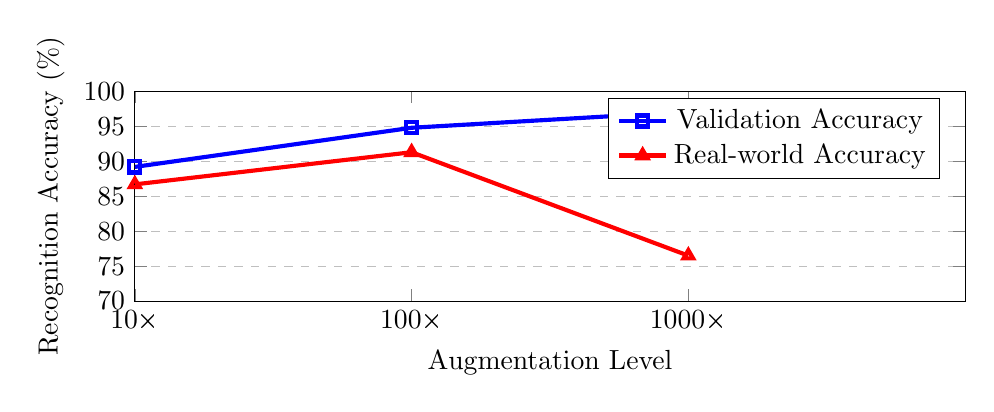
\begin{tikzpicture}
    \begin{axis}[
        width=\columnwidth, % Set width to column width
        height=0.35\textwidth,
        xlabel={Augmentation Level},
        ylabel={Recognition Accuracy (\%)},
        xmin=0, xmax=3,
        ymin=70, ymax=100,
        xtick={0,1,2},
        xticklabels={10×,100×,1000×},
        ytick={70,75,80,85,90,95,100},
        legend pos=north east,
        ymajorgrids=true,
        grid style=dashed,
    ]
    
    \addplot[
        color=blue,
        mark=square,
        line width=1.5pt,
        ]
        coordinates {
        (0,89.2)(1,94.8)(2,97.1)
        };
        \addlegendentry{Validation Accuracy}
        
    \addplot[
        color=red,
        mark=triangle,
        line width=1.5pt,
        ]
        coordinates {
        (0,86.7)(1,91.3)(2,76.5)
        };
        \addlegendentry{Real-world Accuracy}
        
    \end{axis}
    \end{tikzpicture}
    \caption{Recognition accuracy as a function of augmentation level. Note the significant drop in real-world performance at 1000× augmentation despite improved validation accuracy.}
    \label{fig:augmentation_accuracy}
    \end{figure}

Our analysis revealed several key insights:

\begin{enumerate}
\item \textbf{Improvement from 10× to 100×:} Increasing augmentation from 10× to 100× resulted in a significant improvement in both validation accuracy (89.2\% to 94.8\%) and real-world accuracy (86.7\% to 91.3\%). This demonstrates the benefit of moderate data augmentation in enhancing model generalization.

\item \textbf{Diminishing returns and performance degradation at 1000×:} While the 1000× augmentation model achieved the highest validation accuracy (97.1\%), its real-world performance dramatically decreased to 76.5\%. This represents a clear case of overfitting, where the model excels on validation data but fails to generalize to unseen real-world conditions. Our real-world testing environment included challenging conditions not fully represented in the validation set, such as variable classroom lighting (fluorescent lights, window glare, shadows), partial face occlusions (masks, hands), and varying camera angles that the 1000× model failed to handle despite its high validation accuracy.

\item \textbf{Computational efficiency:} The training time increased substantially with higher augmentation levels, from 1.5 hours for 10× to 42.6 hours for 1000×. These training times were measured on a system with an NVIDIA GeForce RTX 2050 4GB GDDR6 GPU and an 11th Gen Intel Core i5-1135G7 processor. We used a batch size of 32 for the 10× and 100× models, but had to reduce to 16 for the 1000× model due to memory constraints, which partially explains the non-linear scaling between dataset size and training time. The 100× augmentation level offered the best balance between performance gain and computational cost.
\end{enumerate}

\subsubsection{Theoretical Analysis}
The observed pattern can be explained through several theoretical frameworks:

\begin{itemize}
\item \textbf{Bias-Variance Tradeoff:} The 10× augmentation model suffered from high bias (underfitting), while the 1000× model exhibited high variance (overfitting). The 100× model achieved the optimal balance between bias and variance.

\item \textbf{Model Capacity Saturation:} With 1000× augmentation, the model's capacity became saturated with highly correlated synthetic examples, leading to memorization rather than generalization. This is evidenced by the high validation accuracy but poor real-world performance.

\item \textbf{Augmentation Diversity vs. Redundancy:} At 100× augmentation, each synthetic example contributed meaningful variation. However, at 1000×, the augmentation space became redundant, with many examples being too similar to provide additional learning signal.

\item \textbf{Manifold Distortion:} Excessive augmentation may have distorted the underlying data manifold, creating synthetic examples that deviated too far from the natural face image distribution encountered in real-world scenarios. Our testing revealed that the 1000× model performed particularly poorly under variable lighting conditions and with partial face occlusions that were common in our classroom testing environment but underrepresented in the validation set.
\end{itemize}

\subsubsection{Conclusion}
Our comparative analysis demonstrates that 100× augmentation (100 variations per original image) represents the optimal level for our face recognition system, balancing improved generalization with computational efficiency. This finding highlights the importance of careful calibration of data augmentation strategies, as excessive augmentation can lead to diminished returns and even performance degradation due to overfitting. Based on these results, we adopted the 100× augmentation strategy for our final system implementation.

\subsection{Real-world Performance}
We evaluated the system in a real classroom environment with varying lighting conditions and student positions. The system achieved a recognition accuracy of 91.3\% with a processing speed of 15 frames per second on a standard laptop with a CUDA-capable GPU.
\section{Conclusion}
In this paper, we presented a robust real-time face recognition attendance system built with FaceNet, PyTorch, and OpenCV. The system leverages extensive data augmentation, a custom feature processing pipeline, and a multi-loss training approach to achieve high recognition accuracy in classroom environments.

The key contributions of our work include:

\begin{itemize}
\item A comprehensive data augmentation pipeline that generates 100 variations per face image using nine different augmentation strategies
\item A custom feature processing pipeline that enhances the discriminative power of facial features
\item A multi-loss training approach that combines Softmax, Center Loss, and Triplet Loss
\item A real-time recognition system with confidence thresholds and cooldown periods
\end{itemize}

Future work will focus on improving the system's performance in extreme lighting conditions and with partial face occlusions, as well as extending the system to support mobile devices.

\section*{Acknowledgment}
We would like to thank all the students who participated in the data collection process and provided valuable feedback on the system's performance.

% Bibliography section
\begin{thebibliography}{00}

    \bibitem{b1}
    Y. Taigman, M. Yang, M. Ranzato, and L. Wolf, ``DeepFace: Closing the Gap to Human-Level Performance in Face Verification,'' in \emph{Proc. IEEE Conf. Comput. Vis. Pattern Recognit.}, 2014, pp. 1701--1708. [Online]. Available: \url{https://ieeexplore.ieee.org/document/6909616}
    
    \bibitem{b2}
    F. Schroff, D. Kalenichenko, and J. Philbin, ``FaceNet: A Unified Embedding for Face Recognition and Clustering,'' in \emph{Proc. IEEE Conf. Comput. Vis. Pattern Recognit.}, 2015, pp. 815--823. [Online]. Available: \url{https://ieeexplore.ieee.org/document/7298682}
    
    \bibitem{b3}
    K. Zhang, Z. Zhang, Z. Li, and Y. Qiao, ``Joint Face Detection and Alignment Using Multitask Cascaded Convolutional Networks,'' \emph{IEEE Signal Process. Lett.}, vol. 23, no. 10, pp. 1499--1503, Oct. 2016. [Online]. Available: \url{https://ieeexplore.ieee.org/document/7553523}
    
    \bibitem{b4}
    J. Deng, J. Guo, N. Xue, and S. Zafeiriou, ``ArcFace: Additive Angular Margin Loss for Deep Face Recognition,'' in \emph{Proc. IEEE Conf. Comput. Vis. Pattern Recognit.}, 2019, pp. 4690--4699. [Online]. Available: \url{https://ieeexplore.ieee.org/document/8953658}
    
    \bibitem{b5}
    W. Liu, Y. Wen, Z. Yu, M. Li, B. Raj, and L. Song, ``SphereFace: Deep Hypersphere Embedding for Face Recognition,'' in \emph{Proc. IEEE Conf. Comput. Vis. Pattern Recognit.}, 2017, pp. 212--220. [Online]. Available: \url{https://ieeexplore.ieee.org/document/8100196}
    
    \bibitem{b6}
    H. Wang, Y. Wang, Z. Zhou, X. Ji, D. Gong, J. Zhou, Z. Li, and W. Liu, ``CosFace: Large Margin Cosine Loss for Deep Face Recognition,'' in \emph{Proc. IEEE Conf. Comput. Vis. Pattern Recognit.}, 2018, pp. 5265--5274. [Online]. Available: \url{https://ieeexplore.ieee.org/document/8578650}
    
    \bibitem{b7}
    Q. Cao, L. Shen, W. Xie, O. M. Parkhi, and A. Zisserman, ``VGGFace2: A Dataset for Recognising Faces across Pose and Age,'' in \emph{Proc. IEEE Int. Conf. Autom. Face Gesture Recognit.}, 2018, pp. 67--74. [Online]. Available: \url{https://ieeexplore.ieee.org/document/8373813}
    
    \end{thebibliography}

\end{document}